\documentclass[12pt,a4paper]{article}
\usepackage[utf8]{inputenc}
\usepackage[T1]{fontenc}
\usepackage[spanish,es-tabla]{babel}
\usepackage[margin=2.5cm]{geometry}
\usepackage{graphicx,xcolor,hyperref,listings,booktabs,longtable,array,ragged2e}
\usepackage{caption,float,pdflscape,fancyhdr,microtype,xurl}
\definecolor{utecblue}{RGB}{0,153,204}
\definecolor{codegray}{RGB}{245,245,245}
\definecolor{tablehead}{RGB}{51,63,72}
\hypersetup{hypertexnames=false,colorlinks=true,linkcolor=utecblue,urlcolor=utecblue,citecolor=utecblue,pdftitle={Kiwi Informe final DevSecOps},pdfauthor={Aarón Timaná Castro; Jean Piero Huaylla Huillca; Mateo Espinoza Monti}}
\urlstyle{same}
\setlength{\emergencystretch}{3em}
\setlength{\parindent}{0pt}
\setlength{\parskip}{7pt}
\setlength{\headheight}{15pt}
\pagestyle{fancy}\fancyhf{}
\fancyhead[L]{\small\textit{Proyecto DevSecOps --- UTEC}}
\fancyhead[R]{\small\textit{Kiwi}}
\fancyfoot[C]{\thepage}\renewcommand{\headrulewidth}{0.4pt}
\captionsetup{font=small,labelfont=bf}
\lstset{backgroundcolor=\color{codegray},basicstyle=\ttfamily\scriptsize,breaklines=true,breakatwhitespace=false,columns=fullflexible,keepspaces=true,showstringspaces=false,frame=single,rulecolor=\color{gray!30},tabsize=2,
literate={á}{{\'a}}1 {é}{{\'e}}1 {í}{{\'i}}1 {ó}{{\'o}}1 {ú}{{\'u}}1 {ñ}{{\~n}}1 {Á}{{\'A}}1 {É}{{\'E}}1 {Í}{{\'I}}1 {Ó}{{\'O}}1 {Ú}{{\'U}}1 {Ñ}{{\~N}}1 {ü}{{\"u}}1 {·}{{$\cdot$}}1 {─}{{-}}1}
\begin{document}
\begin{titlepage}
\centering\vspace*{0.5cm}
\begin{minipage}{0.22\textwidth}\centering

\includegraphics[width=\textwidth]{assets/logo.png}
\end{minipage}\hfill
\begin{minipage}{0.74\textwidth}\raggedright
{\Large\textbf{UNIVERSIDAD DE INGENIERÍA Y TECNOLOGÍA}}\\[0.3cm]
{\large Facultad de Ciencias de la Computación}
\end{minipage}
\par\vspace{2cm}
\rule{\textwidth}{1.5pt}\\[0.4cm]
{\huge\bfseries\color{utecblue} Kiwi\par}
\vspace{0.3cm}
{\Large\itshape Informe final DevSecOps}\\[0.4cm]
\rule{\textwidth}{1.5pt}\\[2cm]
{\Large\textbf{Curso:} IS4024 DevOps}\\[0.6cm]
{\Large\textbf{Profesor:}}\\
{\large Wilson Julca Mejía}\\[1cm]
{\Large\textbf{Integrantes:}}\\[0.4cm]
{\large\begin{tabular}{l}
Timaná Castro, Aarón Víctor Manuel\\
Huaylla Huillca, Jean Piero\\
Espinoza Monti, Mateo
\end{tabular}}\\[1.5cm]
\vfill{\large Lima, Perú\\22 de noviembre de 2026}
\end{titlepage}
\renewcommand{\contentsname}{\textcolor{utecblue}{Índice}}
\tableofcontents
\clearpage

\phantomsection\section*{a Descripción del proyecto}\addcontentsline{toc}{section}{a Descripción del proyecto}
Kiwi es una plataforma de refuerzo educativo para Comunicación de primero de secundaria. El informe parcial del equipo vincula el problema con dificultades de comprensión, expresión y acceso a dispositivos en la I.E. Fe y Alegría. La solución permite administrar aulas, crear y resolver quizzes, registrar resultados y usar recompensas gamificadas. Esta revisión comprueba su implementación técnica y sus controles de seguridad, sin atribuirle resultados pedagógicos que no se han medido.\par
El stack implementado combina Next.js, un gateway FastAPI y microservicios de usuarios en Spring Boot, aulas en Express y Prisma, y quizzes en FastAPI. PostgreSQL almacena los datos. Gemini permite generar contenido desde texto o PDF. El asistente por WhatsApp aparece como intención del informe parcial y no forma parte de la validación realizada en este cierre. La actualización usa Spring Boot 4.0.10 y mantiene Java 17.\par
{\small\setlength{\tabcolsep}{4pt}\renewcommand{\arraystretch}{1.18}
\begin{longtable}{>{\RaggedRight\arraybackslash}p{\dimexpr 0.19321\linewidth-1.15923\tabcolsep\relax}>{\RaggedRight\arraybackslash}p{\dimexpr 0.47159\linewidth-2.82954\tabcolsep\relax}>{\RaggedRight\arraybackslash}p{\dimexpr 0.33520\linewidth-2.01122\tabcolsep\relax}}
\toprule
\textbf{Componente} & \textbf{Responsabilidad} & \textbf{Exposición} \\
\midrule\endfirsthead
\toprule
\textbf{Componente} & \textbf{Responsabilidad} & \textbf{Exposición} \\
\midrule\endhead
\bottomrule\endfoot
Frontend & Interfaz de estudiantes y docentes & Puerto 5174 \\[3pt]
Gateway & Entrada REST y controles de autorización & Puerto 8000 \\[3pt]
ms-user & Registro, perfiles y JWT & Red interna backend \\[3pt]
ms-classroom & Aulas y relaciones & Red interna backend \\[3pt]
ms-quiz & Quizzes y generación con IA & Red interna backend \\[3pt]
PostgreSQL & Persistencia compartida & Red data interna \\[3pt]
\end{longtable}}
La red data está marcada como internal y la base de datos no publica puertos al host. La revisión local usa datos ficticios y claves nuevas. La generación efectiva con Gemini y el envío SMTP no se validaron porque requieren credenciales propias. El E2E cubre perfiles y controles de seguridad, sin acreditar todos los flujos de negocio, capacidad concurrente ni operación productiva.\par
\clearpage\newgeometry{margin=1.5cm}
\begin{landscape}
\phantomsection\section*{b Modelo de amenazas STRIDE}\addcontentsline{toc}{section}{b Modelo de amenazas STRIDE}
El DFD de Kiwi se construyó a partir de compose.yml y del código de los microservicios. Separa siete fronteras de confianza: GitHub, AWS Amplify, dispositivo del usuario, AWS EC2 con Docker Compose, red data interna, Gmail y Gemini. Sobre él se identifican 17 amenazas (T1--T17); seis, una por categoría STRIDE, se priorizan y evalúan con la plantilla del curso: riesgo inherente, efectividad del control y riesgo residual frente a un apetito 3 - Moderate. El diagrama describe la línea base; el estado actual de cada amenaza figura en la sección c.\par
\begin{figure}[H]\centering
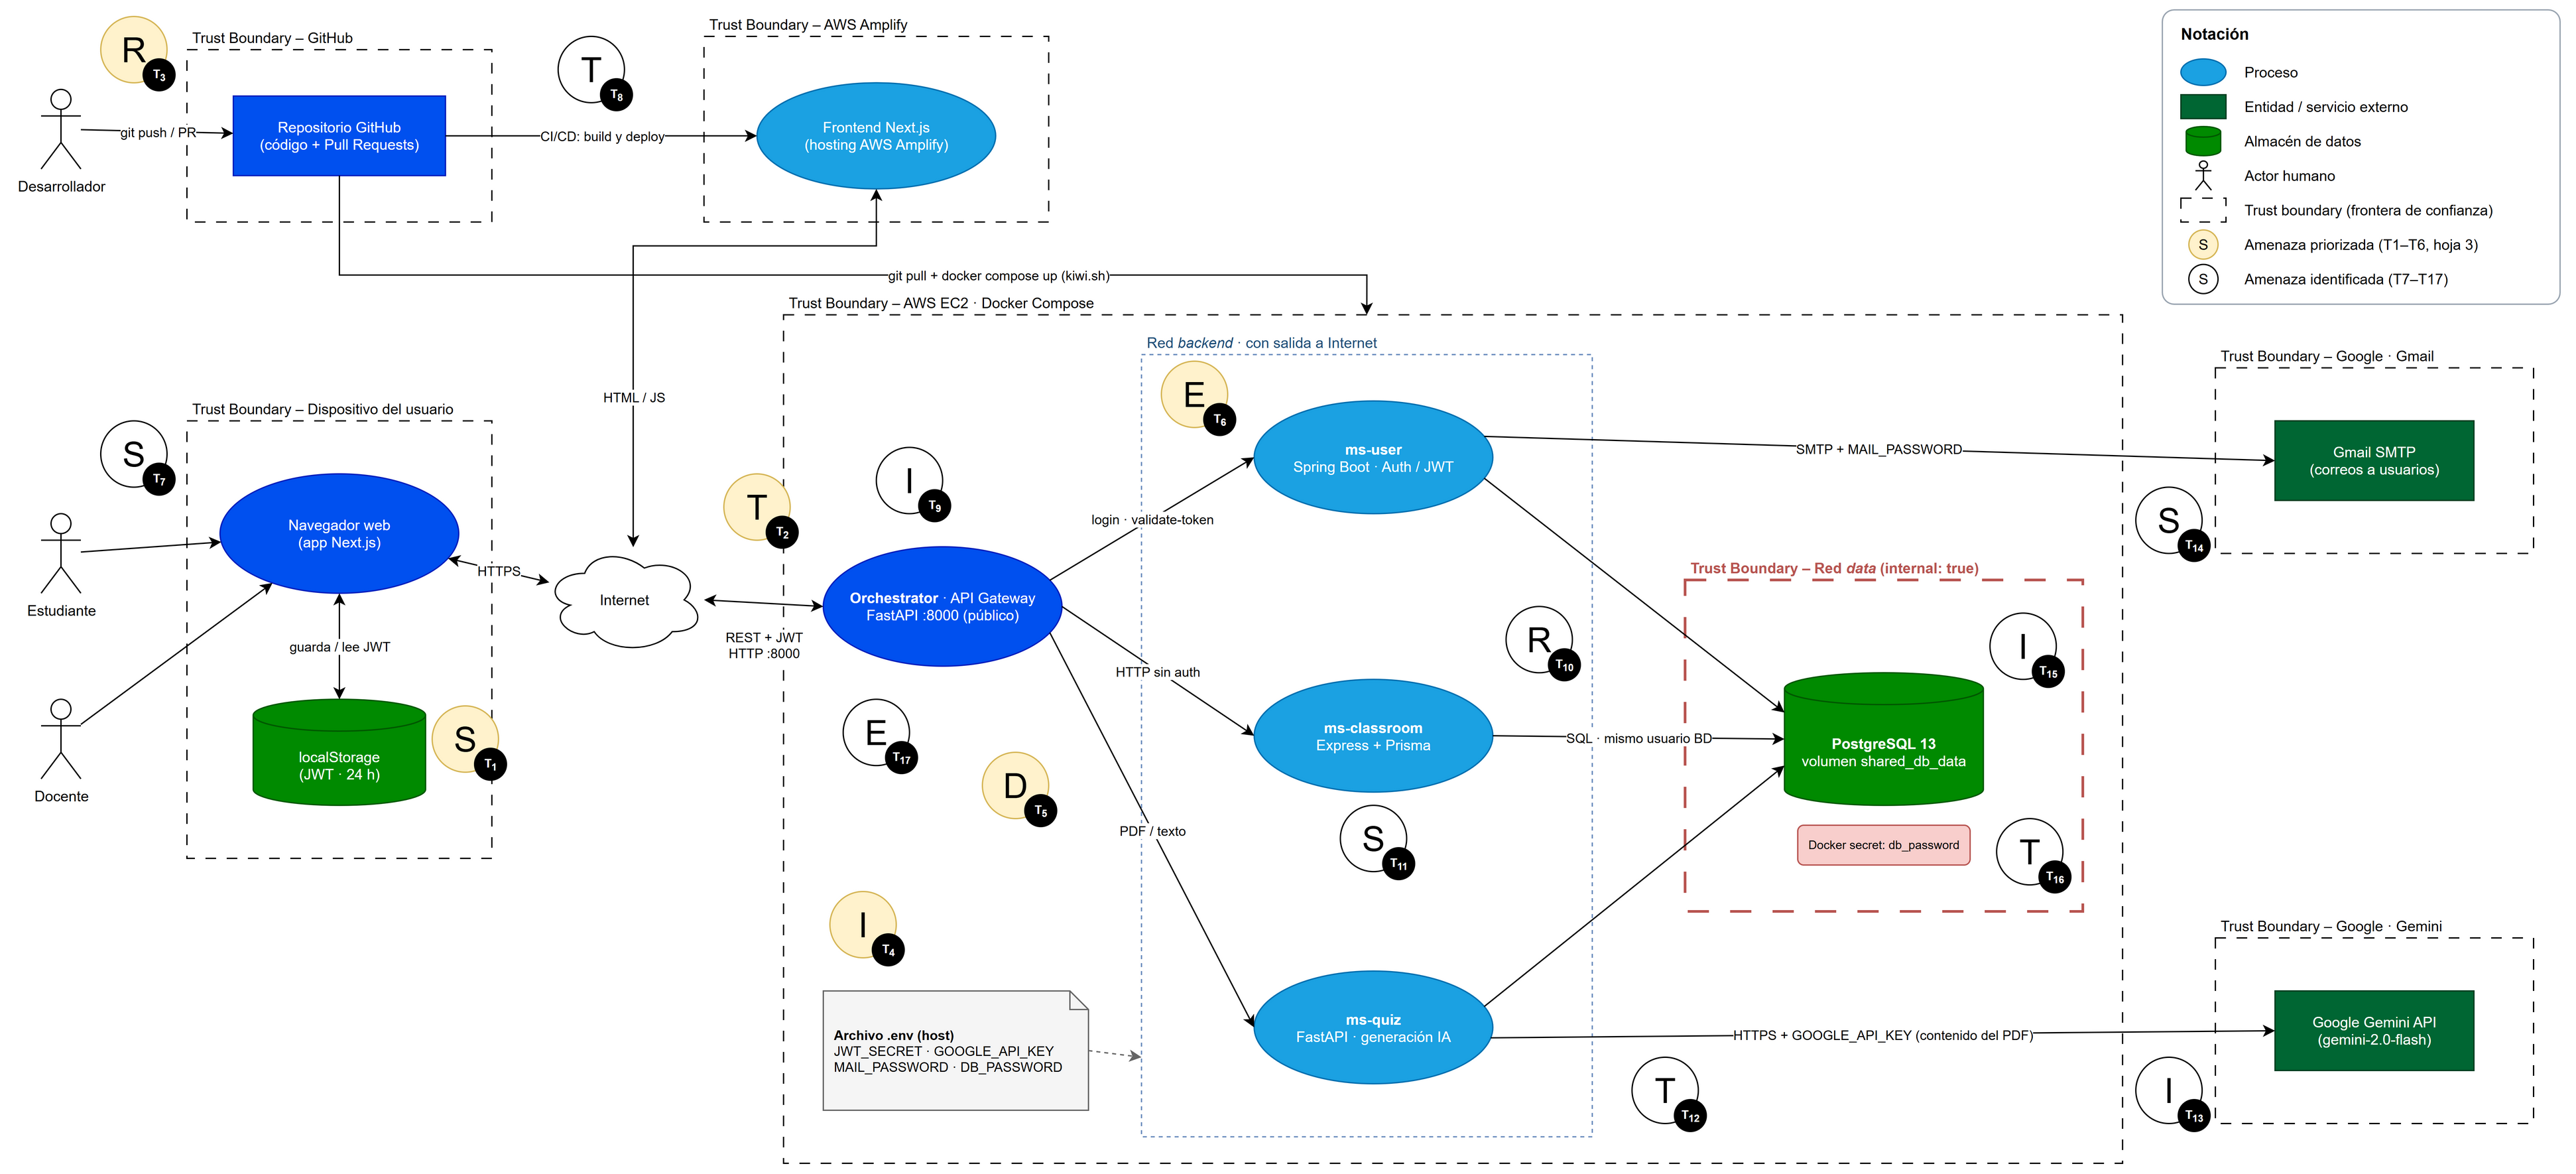
\includegraphics[width=\linewidth,height=0.72\textheight,keepaspectratio]{assets/figura-1.png}
\caption{DFD de Kiwi con las 17 amenazas STRIDE; en amarillo, las seis priorizadas. Fuente editable: kiwi\_stride.drawio (hojas de arquitectura, amenazas y plantilla).}
\end{figure}
\end{landscape}
\restoregeometry
\phantomsection\section*{c Amenazas principales STRIDE}\addcontentsline{toc}{section}{c Amenazas principales STRIDE}
Se explican las seis amenazas priorizadas del diagrama, una por categoría STRIDE. Entre paréntesis se indica el ID equivalente en el Excel del equipo. La evaluación de la plantilla corresponde a la línea base; el estado se verificó en el código del cierre.\par
\phantomsection\subsection*{T1 Spoofing: sesión JWT en el navegador}\addcontentsline{toc}{subsection}{T1 Spoofing: sesión JWT en el navegador}
Riesgo inherente 4 - High, residual 3 - Moderate (S-02). El frontend guarda el JWT en localStorage durante 24 horas y no puede revocarlo; un XSS o un equipo compartido permiten reutilizarlo para suplantar a un docente o estudiante. Se rotó JWT\_SECRET en la computadora revisada y el token anterior devuelve 401. Estado: pendiente; falta mover el token a una cookie HttpOnly, acortar su vigencia y añadir MFA para docentes.\par
\phantomsection\subsection*{T2 Tampering: HTTP sin TLS hacia el gateway}\addcontentsline{toc}{subsection}{T2 Tampering: HTTP sin TLS hacia el gateway}
Riesgo inherente y residual 3 - Moderate. El gateway se publica en el puerto 8000 por HTTP y el compose no incluye terminación TLS, por lo que un atacante en la red puede alterar respuestas, notas o envíos de quiz. Estado: pendiente; se recomienda un proxy con TLS y HSTS y cerrar el puerto 8000 al exterior.\par
\phantomsection\subsection*{T3 Repudiation: commits sin firma}\addcontentsline{toc}{subsection}{T3 Repudiation: commits sin firma}
Riesgo inherente 4 - High, residual 3 - Moderate. Los Pull Requests dejan trazabilidad parcial, pero los commits no están firmados y no hay revisión obligatoria verificable antes del despliegue. Estado: pendiente; requiere firma GPG o SSH, protección de main y CODEOWNERS.\par
\phantomsection\subsection*{T4 Information Disclosure: secretos en variables de entorno}\addcontentsline{toc}{subsection}{T4 Information Disclosure: secretos en variables de entorno}
Riesgo inherente y residual 4 - High (S-01, HIGH-001). JWT\_SECRET, GOOGLE\_API\_KEY y MAIL\_PASSWORD llegan como variables de entorno; solo la contraseña de PostgreSQL usa Docker secrets. Gitleaks conserva 46 ocurrencias históricas de JWT en colecciones Bruno. Estado: parcial; el árbol actual usa variables y la clave local se rotó, pero faltan un gestor de secretos y la rotación confirmada en todos los entornos.\par
\phantomsection\subsection*{T5 Denial of Service: PDF y cuota de IA}\addcontentsline{toc}{subsection}{T5 Denial of Service: PDF y cuota de IA}
Riesgo inherente y residual 3 - Moderate (D-01, MED-002). La generación desde PDF leía el archivo completo y consumía cuota de Gemini en cada petición. Ahora ms-quiz usa pypdf y limita el archivo a 5 MB y 30 páginas, con seis pruebas de límites. Estado: parcial; falta rate limiting por usuario y control de cuota de IA.\par
\phantomsection\subsection*{T6 Elevation of Privilege: registro con rol docente}\addcontentsline{toc}{subsection}{T6 Elevation of Privilege: registro con rol docente}
Riesgo inherente y residual de línea base 4 - High (E-02, HIGH-004). El cliente elegía el rol TEACHER al registrarse. El servidor exige ahora un código de invitación para docentes y las pruebas E2E muestran 403 sin código válido. Estado: mitigado; la custodia del código es una responsabilidad operativa. La amenaza relacionada T17, IDs ajenos en compras e intentos, está mitigada en las rutas cubiertas (HIGH-003).\par
\phantomsection\section*{d Herramientas SAST y DAST}\addcontentsline{toc}{section}{d Herramientas SAST y DAST}
Semgrep revisa patrones en Python, JavaScript, TypeScript, Java y Dockerfiles. Bandit complementa el análisis de los servicios Python. Ambos generan JSON y se ejecutan en jobs de GitHub Actions. SonarCloud es opcional: el run histórico registra que SONAR\_TOKEN no está configurado. Su job verde no acredita que el análisis Sonar se haya ejecutado.\par
OWASP ZAP ejecuta un API scan contra OpenAPI del gateway y un baseline del frontend sobre staging efímero. El workflow registra un usuario docente con invitación y transmite su token al escáner. En el cierre se elimina el fallback silencioso a un análisis sin autenticación. Si no obtiene el token, el job falla.\par
{\small\setlength{\tabcolsep}{4pt}\renewcommand{\arraystretch}{1.18}
\begin{longtable}{>{\RaggedRight\arraybackslash}p{\dimexpr 0.17046\linewidth-1.36366\tabcolsep\relax}>{\RaggedRight\arraybackslash}p{\dimexpr 0.17046\linewidth-1.36366\tabcolsep\relax}>{\RaggedRight\arraybackslash}p{\dimexpr 0.17046\linewidth-1.36366\tabcolsep\relax}>{\RaggedRight\arraybackslash}p{\dimexpr 0.48863\linewidth-3.90901\tabcolsep\relax}}
\toprule
\textbf{Herramienta} & \textbf{Inicial CI} & \textbf{Posterior CI} & \textbf{Interpretación} \\
\midrule\endfirsthead
\toprule
\textbf{Herramienta} & \textbf{Inicial CI} & \textbf{Posterior CI} & \textbf{Interpretación} \\
\midrule\endhead
\bottomrule\endfoot
Semgrep & 49 & 1 & Desaparecen los tokens del árbol y patrones corregidos \\[3pt]
Bandit & 12 & 12 & Persisten hallazgos que requieren triage \\[3pt]
ZAP & 22 & 16 & La cobertura inicial oficial no era autenticada \\[3pt]
\end{longtable}}
El run adicional 44966862163 demuestra DAST autenticado y detecta el hash BCrypt en el perfil con la regla 10097. Esa alerta no aparece en el reporte posterior autenticado. Esta evidencia permite verificar el control de serialización de contraseñas. Los conteos ZAP representan alertas agrupadas, no todas las instancias HTTP individuales.\par
\phantomsection\section*{e Secret scanning y SCA}\addcontentsline{toc}{section}{e Secret scanning y SCA}
Gitleaks analiza el historial completo con redacción. Trivy revisa dependencias del filesystem, configuración e imágenes de los cinco servicios. pip-audit revisa las dependencias declaradas de Python. Los reportes se conservan como artefactos y el resumen normaliza sus severidades. No se suman estos números como si fueran vulnerabilidades únicas: un mismo aviso puede aparecer en filesystem e imagen, o en varias imágenes.\par
Las acciones de terceros del workflow están fijadas por SHA. Los scripts verifican checksums al descargar Gitleaks y Trivy. Persisten tags mutables en algunas imágenes y reglas externas de escáneres, por lo que la reproducibilidad es parcial. Los reportes originales y sus hashes permiten auditar la comparación histórica.\par
{\small\setlength{\tabcolsep}{4pt}\renewcommand{\arraystretch}{1.18}
\begin{longtable}{>{\RaggedRight\arraybackslash}p{\dimexpr 0.34095\linewidth-2.04570\tabcolsep\relax}>{\RaggedRight\arraybackslash}p{\dimexpr 0.32952\linewidth-1.97715\tabcolsep\relax}>{\RaggedRight\arraybackslash}p{\dimexpr 0.32952\linewidth-1.97715\tabcolsep\relax}}
\toprule
\textbf{Herramienta} & \textbf{Inicial CI} & \textbf{Posterior CI} \\
\midrule\endfirsthead
\toprule
\textbf{Herramienta} & \textbf{Inicial CI} & \textbf{Posterior CI} \\
\midrule\endhead
\bottomrule\endfoot
Gitleaks & 48 & 46 \\[3pt]
Trivy & 1063 & 597 \\[3pt]
pip-audit & 1 & 0 \\[3pt]
Checkov & 3 & 0 \\[3pt]
\end{longtable}}
\phantomsection\section*{f Centralización en DefectDojo}\addcontentsline{toc}{section}{f Centralización en DefectDojo}
Se levantó una instancia propia de DefectDojo en localhost:8080 y se importaron los 15 reportes de la línea base. Se reimportaron luego los runs 44972251652 y 45067822680 en el mismo producto Kiwi y engagement CI/CD main. Los 15 tests conservaron sus IDs. La tabla compara la importación inicial con el cierre de referencia.\par
{\small\setlength{\tabcolsep}{4pt}\renewcommand{\arraystretch}{1.18}
\begin{longtable}{>{\RaggedRight\arraybackslash}p{\dimexpr 0.24436\linewidth-3.42107\tabcolsep\relax}>{\RaggedRight\arraybackslash}p{\dimexpr 0.12499\linewidth-1.74982\tabcolsep\relax}>{\RaggedRight\arraybackslash}p{\dimexpr 0.12499\linewidth-1.74982\tabcolsep\relax}>{\RaggedRight\arraybackslash}p{\dimexpr 0.12499\linewidth-1.74982\tabcolsep\relax}>{\RaggedRight\arraybackslash}p{\dimexpr 0.12499\linewidth-1.74982\tabcolsep\relax}>{\RaggedRight\arraybackslash}p{\dimexpr 0.12499\linewidth-1.74982\tabcolsep\relax}>{\RaggedRight\arraybackslash}p{\dimexpr 0.13070\linewidth-1.82981\tabcolsep\relax}}
\toprule
\textbf{Estado} & \textbf{Critical} & \textbf{High} & \textbf{Medium} & \textbf{Low} & \textbf{Info} & \textbf{Total} \\
\midrule\endfirsthead
\toprule
\textbf{Estado} & \textbf{Critical} & \textbf{High} & \textbf{Medium} & \textbf{Low} & \textbf{Info} & \textbf{Total} \\
\midrule\endhead
\bottomrule\endfoot
Antes importado & 33 & 381 & 485 & 276 & 22 & 1197 \\[3pt]
Cierre activo & 0 & 156 & 286 & 195 & 35 & 672 \\[3pt]
\end{longtable}}
La instancia propia conserva 15 tests y 1233 registros históricos después de todas las importaciones. El estado actual tiene 672 activos y 561 mitigados. Se crearon 36 registros adicionales a lo largo de las reimportaciones. Las diferencias LOW e INFO frente al CSV corresponden al parser. Las propuestas de aceptación de riesgos permanecen pendientes de decisión del equipo.\par
\begin{figure}[H]\centering
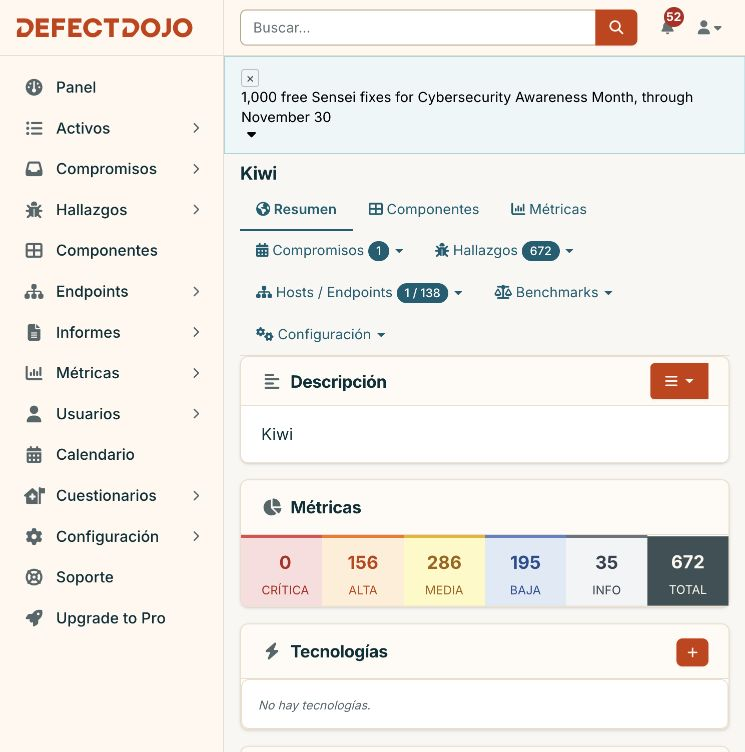
\includegraphics[width=\linewidth,height=0.60\textheight,keepaspectratio]{assets/figura-2.png}
\caption{Producto Kiwi después de reimportar el run de código de referencia. Captura real de la instancia propia.}
\end{figure}
\clearpage
\phantomsection\section*{g Tabla de mitigaciones}\addcontentsline{toc}{section}{g Tabla de mitigaciones}
La rúbrica requiere al menos cinco hallazgos priorizados. La tabla resume siete y el Excel conserva las 20 filas originales con sus estados. Las mitigaciones de Spring, Tomcat y del contrato PATCH se confirmaron en CI. Los estados parciales conservan controles o decisiones aún abiertos.\par
{\small\setlength{\tabcolsep}{4pt}\renewcommand{\arraystretch}{1.18}
\begin{longtable}{>{\RaggedRight\arraybackslash}p{\dimexpr 0.13070\linewidth-1.30701\tabcolsep\relax}>{\RaggedRight\arraybackslash}p{\dimexpr 0.25569\linewidth-2.55688\tabcolsep\relax}>{\RaggedRight\arraybackslash}p{\dimexpr 0.13070\linewidth-1.30701\tabcolsep\relax}>{\RaggedRight\arraybackslash}p{\dimexpr 0.17611\linewidth-1.76105\tabcolsep\relax}>{\RaggedRight\arraybackslash}p{\dimexpr 0.30681\linewidth-3.06806\tabcolsep\relax}}
\toprule
\textbf{ID} & \textbf{Descripción} & \textbf{Severidad} & \textbf{Herramienta} & \textbf{Recomendación y estado} \\
\midrule\endfirsthead
\toprule
\textbf{ID} & \textbf{Descripción} & \textbf{Severidad} & \textbf{Herramienta} & \textbf{Recomendación y estado} \\
\midrule\endhead
\bottomrule\endfoot
CRIT-001 & Next.js vulnerable en el frontend & CRITICAL & Trivy / npm audit & Actualizar Next y reconstruir. Mitigado para los avisos de línea base. \\[3pt]
CRIT-005 & Tomcat embebido desactualizado & CRITICAL & Trivy image & Boot 4.0.10 administra Tomcat 11.0.27 y Spring 7.0.11. Escaneos sin los CRITICAL anteriores. \\[3pt]
HIGH-004 & Alta docente controlada por el cliente & HIGH & Revisión STRIDE & Invitación validada por el servidor. Mitigado y comprobado con E2E. \\[3pt]
HIGH-003 & IDs ajenos en compras e intentos & HIGH & Revisión STRIDE & Identidad del token y respuesta 403. Mitigado en rutas cubiertas. \\[3pt]
HIGH-005 & Hash BCrypt en perfiles & HIGH & ZAP autenticado & Excluir password de las respuestas. Mitigado y comprobado con E2E. \\[3pt]
MED-002 & PDF y lector vulnerable & MEDIUM & pip-audit & Migrar a pypdf y limitar archivos. Dependencia mitigada, cuota IA pendiente. \\[3pt]
LOW-001 & Imágenes sin healthcheck & LOW & Checkov / Trivy & Agregar HEALTHCHECK. Mitigado, seis servicios Kiwi healthy. \\[3pt]
\end{longtable}}
Los hallazgos manuales se identifican como revisión STRIDE y no se atribuyen a un escáner que no los detectó. La comparación conserva las severidades originales de los escáneres; los CRITICAL de Spring se corrigieron actualizando componentes. El detalle está en VALIDACION.md y triage-propuesto.csv.\par
\clearpage
\phantomsection\section*{h Situación inicial y resultados}\addcontentsline{toc}{section}{h Situación inicial y resultados}
{\small\setlength{\tabcolsep}{4pt}\renewcommand{\arraystretch}{1.18}
\begin{longtable}{>{\RaggedRight\arraybackslash}p{\dimexpr 0.26135\linewidth-2.09079\tabcolsep\relax}>{\RaggedRight\arraybackslash}p{\dimexpr 0.22728\linewidth-1.81822\tabcolsep\relax}>{\RaggedRight\arraybackslash}p{\dimexpr 0.22728\linewidth-1.81822\tabcolsep\relax}>{\RaggedRight\arraybackslash}p{\dimexpr 0.28410\linewidth-2.27277\tabcolsep\relax}}
\toprule
\textbf{Severidad} & \textbf{Inicial CI} & \textbf{Final CI} & \textbf{Reducción} \\
\midrule\endfirsthead
\toprule
\textbf{Severidad} & \textbf{Inicial CI} & \textbf{Final CI} & \textbf{Reducción} \\
\midrule\endhead
\bottomrule\endfoot
CRITICAL & 33 & 0 & 100,0 \% \\[3pt]
HIGH & 382 & 156 & 59,2 \% \\[3pt]
MEDIUM & 485 & 286 & 41,0 \% \\[3pt]
LOW & 275 & 194 & 29,5 \% \\[3pt]
INFO & 23 & 36 & -56,5 \% \\[3pt]
Total & 1198 & 672 & 43,9 \% \\[3pt]
CRITICAL y HIGH & 415 & 156 & 62,4 \% \\[3pt]
\end{longtable}}
Los totales se reprodujeron procesando los artefactos descargados de GitHub, con verificación de hashes. Los escaneos inicial y posterior tienen diferencias de cobertura: ZAP oficial inicial no autenticó, mientras que el posterior sí lo hizo. También pueden variar bases de vulnerabilidades, imágenes y dependencias. El porcentaje agregado describe detecciones observadas y no una reducción causal exacta del riesgo ni del número de vulnerabilidades únicas. INFO también agrupa avisos UNKNOWN de Trivy; requiere triage y no equivale a ausencia de riesgo.\par
El run de cierre 45067822680, commit 41aaa61, genera 672 detecciones completas: 0 CRITICAL, 156 HIGH, 286 MEDIUM, 194 LOW y 36 INFO. Todas las pruebas, los escaneos, build, staging, autenticación ZAP y sondas de monitoreo terminaron correctamente. El gate terminó correctamente sin CRITICAL. El release quedó omitido porque la rama no es main. Se validó la construcción y staging, sin acreditar despliegue productivo.\par
Se migró ms-user de Spring Boot 3.5.16 a 4.0.10, con Spring Framework 7.0.11, Tomcat 11.0.27 y PostgreSQL JDBC 42.7.14 administrados por su BOM. Se adaptaron los matchers y constructores de Spring Security y se conservaron los valores JSON de Jackson 2 mediante la opción de compatibilidad de Jackson 3. Los avisos CVE-2026-47884 y CVE-2026-47890 ya no aparecen en el nuevo inventario. No se introdujeron exclusiones ni excepciones de severidad.\par
\phantomsection\section*{i Pipeline completo}\addcontentsline{toc}{section}{i Pipeline completo}
El workflow histórico declara 11 jobs, incluidos SonarCloud opcional y release condicional. El cierre agrega un job JUnit y completa pytest de quiz, por lo que el YAML actual declara 12. El diagrama siguiente se genera desde sus dependencias needs. El release espera también pruebas y escaneos, y el gate exige los 15 JSON esperados antes de consolidar resultados.\par
\begin{figure}[H]\centering
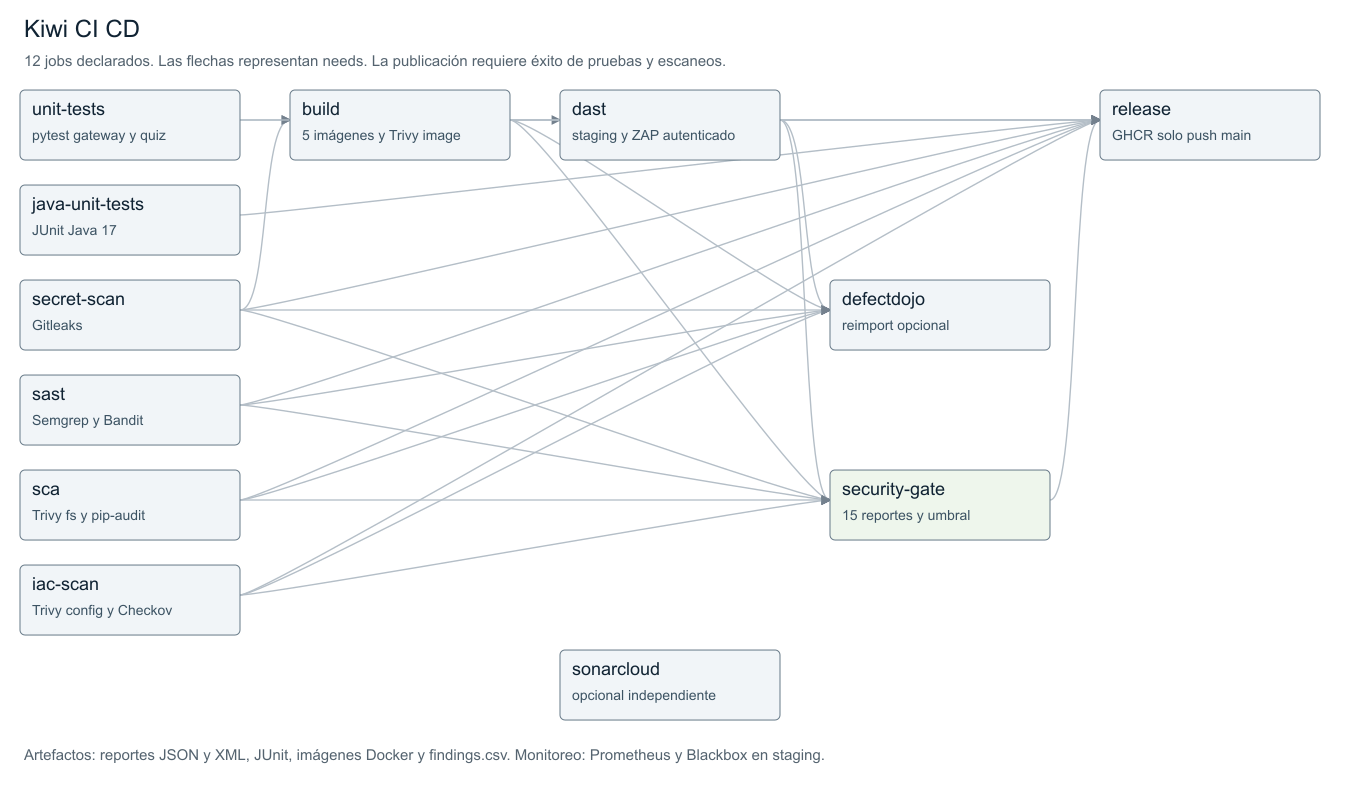
\includegraphics[width=\linewidth,height=0.60\textheight,keepaspectratio]{assets/figura-3.png}
\caption{Dependencias del pipeline preparado para el cierre. El YAML completo figura en el anexo.}
\end{figure}
El umbral predeterminado es CRITICAL y la variable SECURITY\_GATE\_SEVERITY puede endurecerlo a HIGH. El run 45067822680 verifica 15 reportes sin errores y aprueba con cero CRITICAL. Las evidencias conservan el log del gate y la captura del grafo. El run histórico en modo línea base se conserva por separado y no se confunde con esta comprobación.\par
\begin{figure}[H]\centering
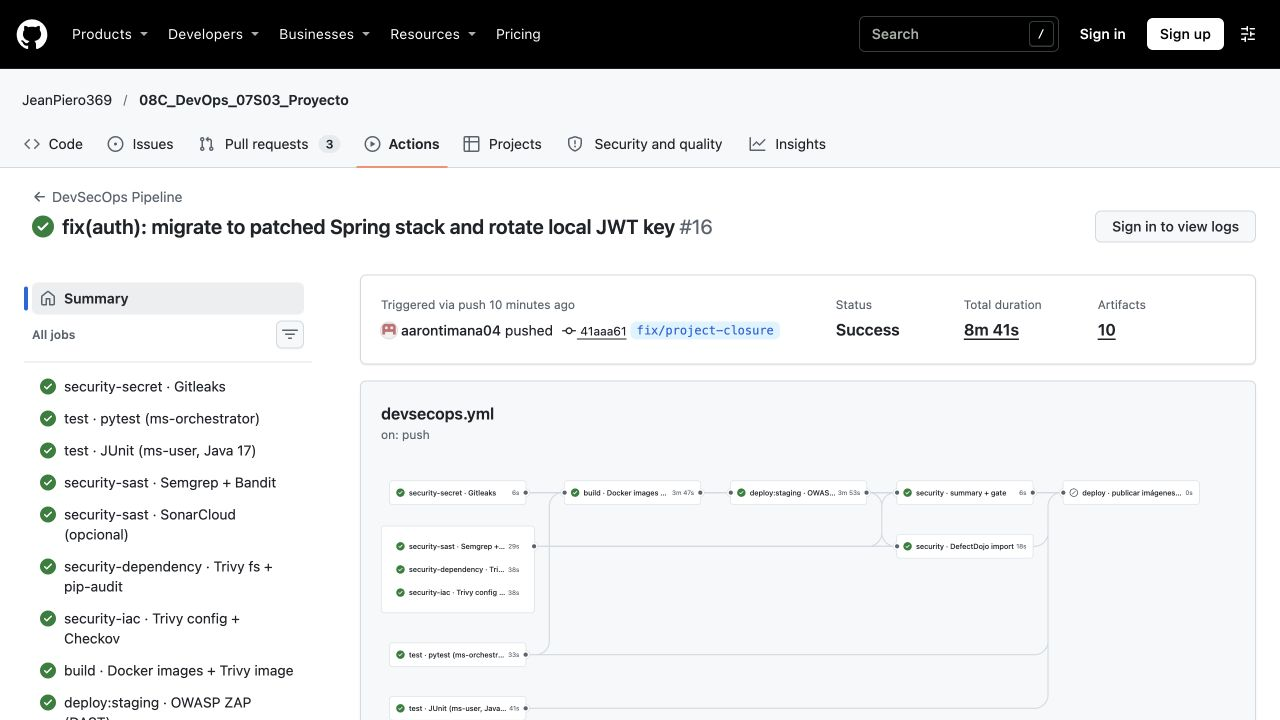
\includegraphics[width=\linewidth,height=0.60\textheight,keepaspectratio]{assets/figura-4.png}
\caption{Run 45067822680: pruebas, análisis y security-gate correctos; release omitido fuera de main.}
\end{figure}
\phantomsection\section*{j Ambientes y monitoreo}\addcontentsline{toc}{section}{j Ambientes y monitoreo}
{\small\setlength{\tabcolsep}{4pt}\renewcommand{\arraystretch}{1.18}
\begin{longtable}{>{\RaggedRight\arraybackslash}p{\dimexpr 0.18749\linewidth-1.12496\tabcolsep\relax}>{\RaggedRight\arraybackslash}p{\dimexpr 0.41477\linewidth-2.48863\tabcolsep\relax}>{\RaggedRight\arraybackslash}p{\dimexpr 0.39774\linewidth-2.38641\tabcolsep\relax}}
\toprule
\textbf{Ambiente} & \textbf{Ejecución y datos} & \textbf{Validación} \\
\midrule\endfirsthead
\toprule
\textbf{Ambiente} & \textbf{Ejecución y datos} & \textbf{Validación} \\
\midrule\endhead
\bottomrule\endfoot
Desarrollo & Compose local con credenciales nuevas y datos ficticios & Pruebas unitarias y 16 comprobaciones E2E \\[3pt]
Staging CI & Compose efímero sobre imágenes construidas & ZAP autenticado, sondas HTTP y reportes \\[3pt]
Distribución & Job de publicación de main en GHCR & Configurado, no ejecutado en este cierre \\[3pt]
Producción & Infraestructura no identificada en el traspaso & Despliegue y operación pendientes \\[3pt]
\end{longtable}}
El perfil monitoring incorpora Prometheus y Blackbox Exporter. Dos sondas consultan el frontend y OpenAPI del gateway cada 15 segundos. probe\_success indica disponibilidad HTTP, y probe\_duration\_seconds mide duración de la sonda. Los healthchecks de Compose revisan el estado de los servicios. Estas señales no reemplazan métricas de negocio ni pruebas de carga.\par
Se validaron configuración y reglas con promtool. En una prueba controlada se detuvo frontend, se observó KiwiEndpointDown en firing después del período definido y se restauró el servicio. Se verificaron las dos sondas sanas y la desaparición de la alerta. KiwiProbeMissing cubre fallos de scraping. No se configuraron notificaciones externas ni se afirma monitoreo productivo permanente.\par
\begin{figure}[H]\centering
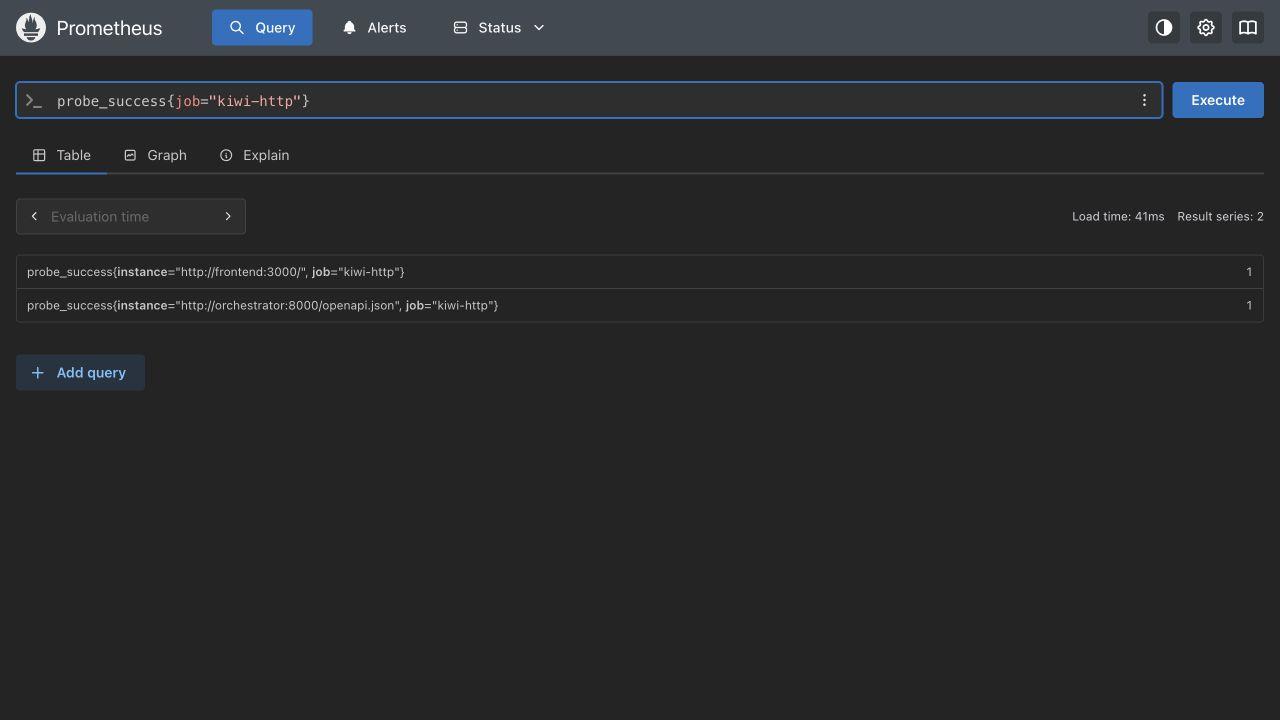
\includegraphics[width=\linewidth,height=0.60\textheight,keepaspectratio]{assets/figura-5.png}
\caption{Dos sondas HTTP reales con resultado 1. Los JSON conservan fallo, alerta y recuperación.}
\end{figure}
\phantomsection\section*{k Modelo de madurez}\addcontentsline{toc}{section}{k Modelo de madurez}
Se usa OWASP SAMM 2 como referencia de madurez de seguridad dentro de DevSecOps. SAMM organiza cinco funciones y quince prácticas. La evaluación es una autoevaluación del proyecto académico, no una certificación ni una puntuación global calculada a partir de un solo pipeline.\par
{\small\setlength{\tabcolsep}{4pt}\renewcommand{\arraystretch}{1.18}
\begin{longtable}{>{\RaggedRight\arraybackslash}p{\dimexpr 0.21024\linewidth-1.26145\tabcolsep\relax}>{\RaggedRight\arraybackslash}p{\dimexpr 0.41477\linewidth-2.48863\tabcolsep\relax}>{\RaggedRight\arraybackslash}p{\dimexpr 0.37499\linewidth-2.24992\tabcolsep\relax}}
\toprule
\textbf{Práctica SAMM} & \textbf{Evidencia} & \textbf{Situación alcanzada} \\
\midrule\endfirsthead
\toprule
\textbf{Práctica SAMM} & \textbf{Evidencia} & \textbf{Situación alcanzada} \\
\midrule\endhead
\bottomrule\endfoot
Threat Assessment & DFD, STRIDE con 17 amenazas y seis priorizadas & Actividades iniciales documentadas \\[3pt]
Secure Build & Build automatizado y análisis de dependencias & Automatización implementada, reproducibilidad parcial \\[3pt]
Defect Management & DefectDojo con reimportación y estados & Seguimiento inicial operativo \\[3pt]
Security Testing & SAST, DAST y pruebas negativas de controles & Objetivo del nivel 1 demostrado en el alcance revisado \\[3pt]
Operations & Sondas y prueba de caída y recuperación & Base local, sin operación productiva sostenida \\[3pt]
\end{longtable}}
El objetivo de nivel 1 de Security Testing consiste en descubrir defectos con herramientas y pruebas manuales. El proyecto aporta ambos tipos de evidencia y automatiza una parte de ellos en CI. No se declara nivel 2 o 3 global: faltan evaluación completa de los flujos de cada práctica, pruebas de penetración regulares, acuerdos operativos, rotación confirmada de claves y mediciones sostenidas. El siguiente ciclo debe ampliar la evaluación SAMM y definir responsables para los controles operativos.\par
\phantomsection\section*{l Lecciones aprendidas}\addcontentsline{toc}{section}{l Lecciones aprendidas}
El problema de negocio es ofrecer refuerzo educativo accesible sin exponer identidades, resultados ni recompensas de los estudiantes. La arquitectura por microservicios permite separar responsabilidades, pero exige mantener contratos, autorización y dependencias de varios stacks.\par
Antes de DevSecOps, las dependencias vulnerables, los JWT versionados y los controles insuficientes de rol e identidad podían entrar al repositorio sin una evaluación conjunta. El primer pipeline y STRIDE hicieron visibles esos riesgos. El DAST autenticado mostró una divulgación de hash que el análisis sin sesión no había revelado.\par
Durante la integración, una dependencia de frontend llegaba de manera indirecta por otro paquete, y dependencias Python sin fijar rompieron el arranque según el registro del equipo. La lección es declarar dependencias reales y validar el stack completo. El cierre corroboró además un PATCH de perfil que no reenviaba el cuerpo: dos pruebas de regresión y un E2E ahora verifican ese contrato.\par
La carrera de arranque de ms-user obligó a esperar disponibilidad antes de registrar el usuario ZAP. Convertir esa falla en un análisis no autenticado reducía cobertura sin fallar el job. El cierre exige autenticación correcta y reportes completos. También mostró que un job verde puede haber omitido SonarCloud o DefectDojo por falta de credenciales.\par
Las ventajas observadas son trazabilidad de hallazgos, validación repetible de controles y menor número de detecciones en los runs comparados. DefectDojo aporta estados de mitigación por reimportación. Prometheus añade señales de disponibilidad y una alerta comprobada. No se atribuyen mejoras de rendimiento, aprendizaje de estudiantes o disponibilidad productiva porque no se midieron.\par
\phantomsection\section*{m Recomendaciones}\addcontentsline{toc}{section}{m Recomendaciones}
Para otros proyectos conviene empezar por un inventario de servicios y un modelo de amenazas ligado a rutas concretas. Las pruebas negativas deben verificar qué ocurre cuando un usuario intenta actuar sobre recursos ajenos. Los escáneres complementan esas pruebas y requieren triage humano para distinguir condiciones aplicables, falsos positivos y riesgos pendientes.\par
El pipeline debe fallar si una herramienta no ejecuta el análisis requerido o falta su reporte. Los umbrales tienen que ser explícitos y la publicación debe depender también de pruebas y builds correctos. La evidencia debe identificar commit, run, versión de herramienta y cobertura de autenticación.\par
La promoción debe separar credenciales y datos de desarrollo, staging y producción. Antes de operar con usuarios reales, hacen falta rotación de secretos, copias y restauración probada, actualización de componentes, autorización por pertenencia y monitoreo con responsables. Los límites de PDF deben complementarse con cuotas y rate limiting de IA.\par
El equipo indicó que usa únicamente computadoras locales. Se rotó JWT\_SECRET en la computadora revisada y se verificó que un token anterior devuelve 401 y que un login nuevo funciona. Cada otro integrante debe ejecutar la rotación local y confirmar el resultado. El cierre requiere revisar el triage residual y acordar la integración. El PR 13 ya contiene los cambios técnicos y sus reportes de CI. Los merges y cualquier purga de historial requieren coordinación con el dueño del repositorio. GHCR representa distribución de imágenes y no acredita una instalación productiva disponible.\par
\clearpage
\clearpage
\phantomsection\section*{Anexo Configuración del pipeline}\addcontentsline{toc}{section}{Anexo Configuración del pipeline}
Archivo .github/workflows/devsecops.yml de la continuación de cierre. Este anexo conserva la configuración completa, incluidas las herramientas opcionales. Los enlaces finales deben apuntar al commit que el equipo publique y valide.\par
\lstinputlisting{devsecops.yml}
\clearpage
\clearpage
\phantomsection\section*{Referencias y enlaces de entrega}\addcontentsline{toc}{section}{Referencias y enlaces de entrega}
Repositorio \url{https://github.com/JeanPiero369/08C_DevOps_07S03_Proyecto}\par
Rama de cierre \url{https://github.com/JeanPiero369/08C_DevOps_07S03_Proyecto/tree/fix/project-closure}\par
Diagrama STRIDE \url{https://github.com/JeanPiero369/08C_DevOps_07S03_Proyecto/blob/fix/project-closure/docs/devsecops/stride/kiwi_stride.drawio}\par
Plantilla STRIDE Excel \url{https://github.com/JeanPiero369/08C_DevOps_07S03_Proyecto/blob/fix/project-closure/docs/devsecops/stride/kiwi_stride.xlsx}\par
Línea base CI \url{https://github.com/JeanPiero369/08C_DevOps_07S03_Proyecto/actions/runs/44965126475}\par
ZAP autenticado adicional \url{https://github.com/JeanPiero369/08C_DevOps_07S03_Proyecto/actions/runs/44966862163}\par
Resultado CI histórico \url{https://github.com/JeanPiero369/08C_DevOps_07S03_Proyecto/actions/runs/44972251652}\par
Tomcat avisos de seguridad \url{https://tomcat.apache.org/security-11.html}\par
Spring XsltView \url{https://spring.io/security/cve-2026-47884/}\par
Spring SSE \url{https://spring.io/security/cve-2026-47890/}\par
Prometheus patrón de sondas \url{https://prometheus.io/docs/guides/multi-target-exporter/}\par
Modelo OWASP SAMM \url{https://owaspsamm.org/model/}\par
SAMM Security Testing \url{https://owaspsamm.org/model/verification/security-testing/}\par
Fuente de requisitos: Proyecto - Informe final.pdf, páginas 1 a 3, suministrado por el equipo. Contexto de negocio: Informe Parcial (1).pdf del repositorio. Evidencias reproducibles: docs/devsecops/cierre y los CSV de baseline-ci y final-ci. La carpeta entrega contiene la versión del informe preparada con estas fuentes.\par
CI de código de referencia \url{https://github.com/JeanPiero369/08C_DevOps_07S03_Proyecto/actions/runs/45067822680}\par
Guía oficial de migración a Boot 4 \url{https://github.com/spring-projects/spring-boot/wiki/Spring-Boot-4.0-Migration-Guide}\par
\end{document}
